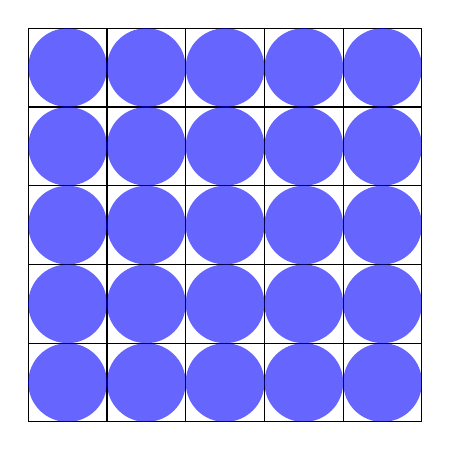
\begin{tikzpicture}
	\draw (0, 0) grid (5, 5);
	\fill[blue, fill opacity=.6] (0.5, 0.5) circle[radius=0.5];
	\fill[blue, fill opacity=.6] (0.5, 1.5) circle[radius=0.5];
	\fill[blue, fill opacity=.6] (0.5, 2.5) circle[radius=0.5];
	\fill[blue, fill opacity=.6] (0.5, 3.5) circle[radius=0.5];
	\fill[blue, fill opacity=.6] (0.5, 4.5) circle[radius=0.5];
	\fill[blue, fill opacity=.6] (1.5, 0.5) circle[radius=0.5];
	\fill[blue, fill opacity=.6] (1.5, 1.5) circle[radius=0.5];
	\fill[blue, fill opacity=.6] (1.5, 2.5) circle[radius=0.5];
	\fill[blue, fill opacity=.6] (1.5, 3.5) circle[radius=0.5];
	\fill[blue, fill opacity=.6] (1.5, 4.5) circle[radius=0.5];
	\fill[blue, fill opacity=.6] (2.5, 0.5) circle[radius=0.5];
	\fill[blue, fill opacity=.6] (2.5, 1.5) circle[radius=0.5];
	\fill[blue, fill opacity=.6] (2.5, 2.5) circle[radius=0.5];
	\fill[blue, fill opacity=.6] (2.5, 3.5) circle[radius=0.5];
	\fill[blue, fill opacity=.6] (2.5, 4.5) circle[radius=0.5];
	\fill[blue, fill opacity=.6] (3.5, 0.5) circle[radius=0.5];
	\fill[blue, fill opacity=.6] (3.5, 1.5) circle[radius=0.5];
	\fill[blue, fill opacity=.6] (3.5, 2.5) circle[radius=0.5];
	\fill[blue, fill opacity=.6] (3.5, 3.5) circle[radius=0.5];
	\fill[blue, fill opacity=.6] (3.5, 4.5) circle[radius=0.5];
	\fill[blue, fill opacity=.6] (4.5, 0.5) circle[radius=0.5];
	\fill[blue, fill opacity=.6] (4.5, 1.5) circle[radius=0.5];
	\fill[blue, fill opacity=.6] (4.5, 2.5) circle[radius=0.5];
	\fill[blue, fill opacity=.6] (4.5, 3.5) circle[radius=0.5];
	\fill[blue, fill opacity=.6] (4.5, 4.5) circle[radius=0.5];
\end{tikzpicture}
